\section{Additional Figures}
\label{sec:appendix2:figures}

\begin{figure*}[bh!]
\centering
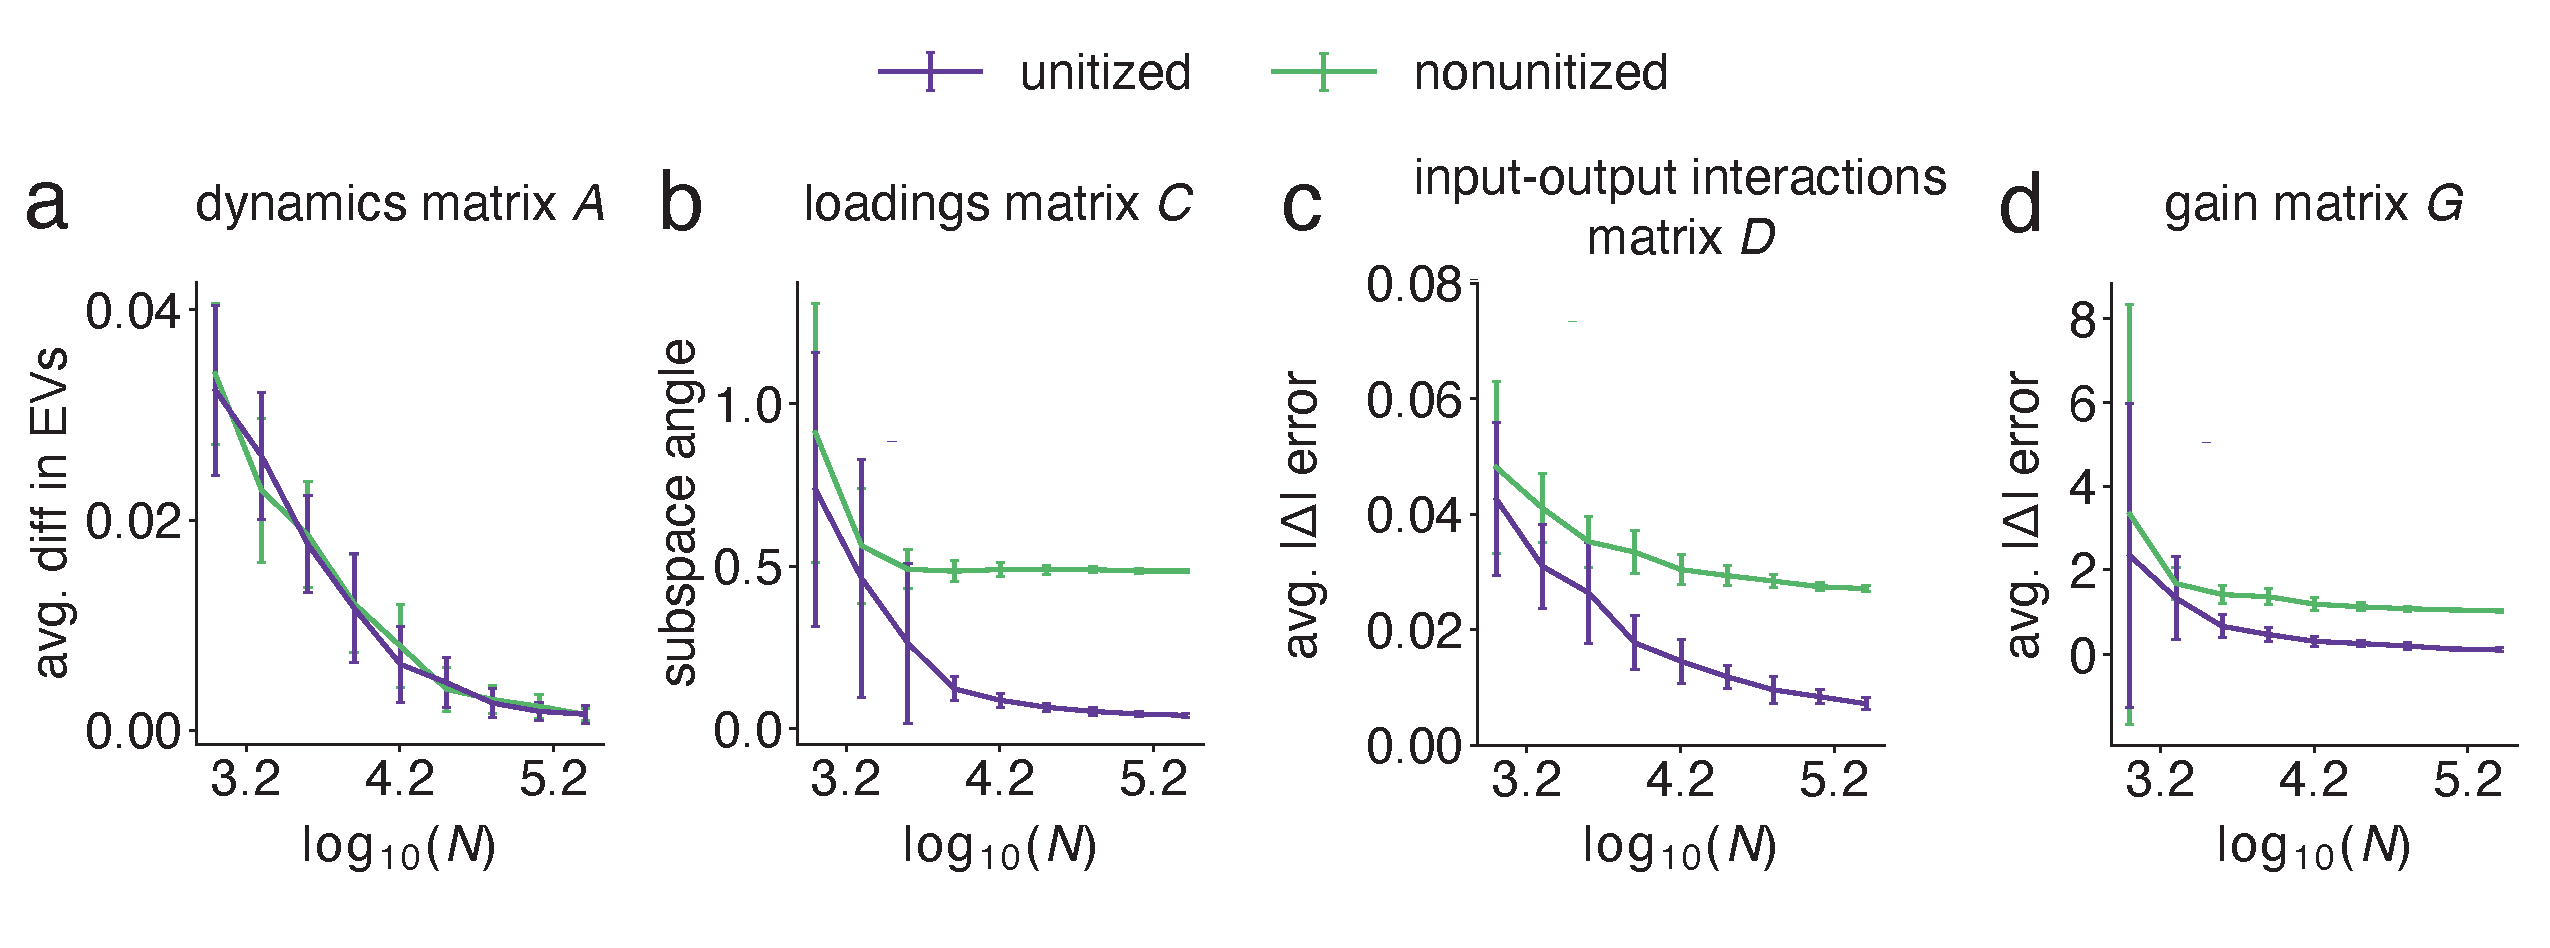
\includegraphics[width=0.90\textwidth]{ch4-bestlds/bestlds-figures/suppfig1.pdf}
\caption[Spectral estimator recovers simulation parameters in a variety of settings]{\textbf{Spectral estimator recovers simulation parameters in a variety of settings.} \textbf{(a)} Covariance matrix Cov$[y_{t+1}, y_{t}]$ showing the sample covariance of the binary observations $y$ (left), the covariance of $z$ obtained by converting the moments of $y$ (middle), and the ground truth covariance of $z$ (right) for a simulated dataset ($q = 30$, $p = 15$, $k =20$, $m=3$). Note that the transformed covariance closely matches the ground truth. \textbf{(b)} The singular value spectrum of the Hankel matrix computed at various settings of the Hankel size $k$. For all settings, only the top $p=5$ singular values are greater than zero. \textbf{(c-e)} Recovery error for bestLDS inferred parameters vs. training data size for a low-dimensional dataset with $ k=3$. For (c) we use the average absolute difference in the eigenvalues as the recovery error, and for (d) and (e) we use the average absolute elementwise difference. \textbf{(f-i)} Recovery error for bestLDS inferred parameters vs. training data size for a high-dimensional dataset with $k=10$. For (g) the recovery error is the angle of the }
%\vspace{-0.5cm}
\label{fig:ap2:1}
\end{figure*}

\begin{figure*}[ht]
\centering
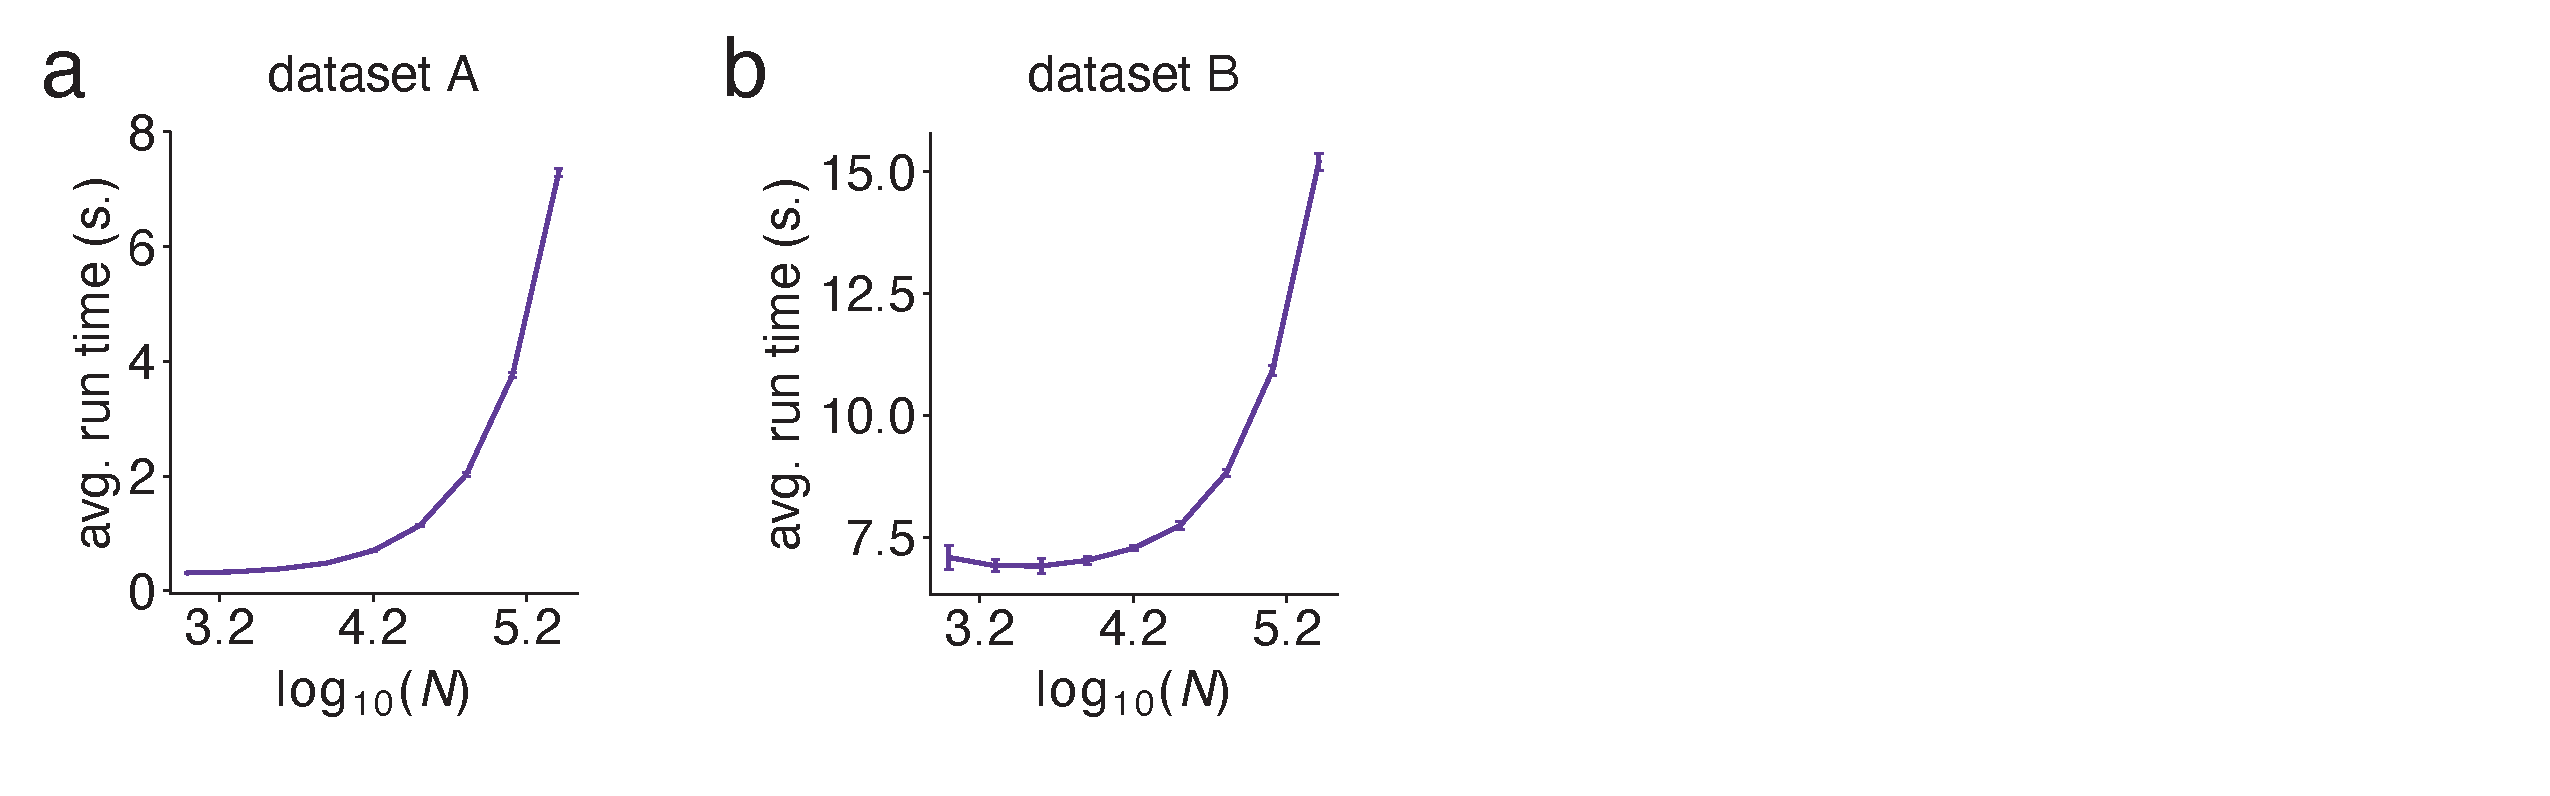
\includegraphics[width=0.90\linewidth]{ch4-bestlds/bestlds-figures/suppfig2.pdf}
\caption[bestLDS run time as a function of dataset size]{\textbf{bestLDS run time as a function of dataset size.}}
\label{fig:ap2:2}
\vspace{-0.5cm}
\end{figure*}

\begin{figure*}[t]
\centering
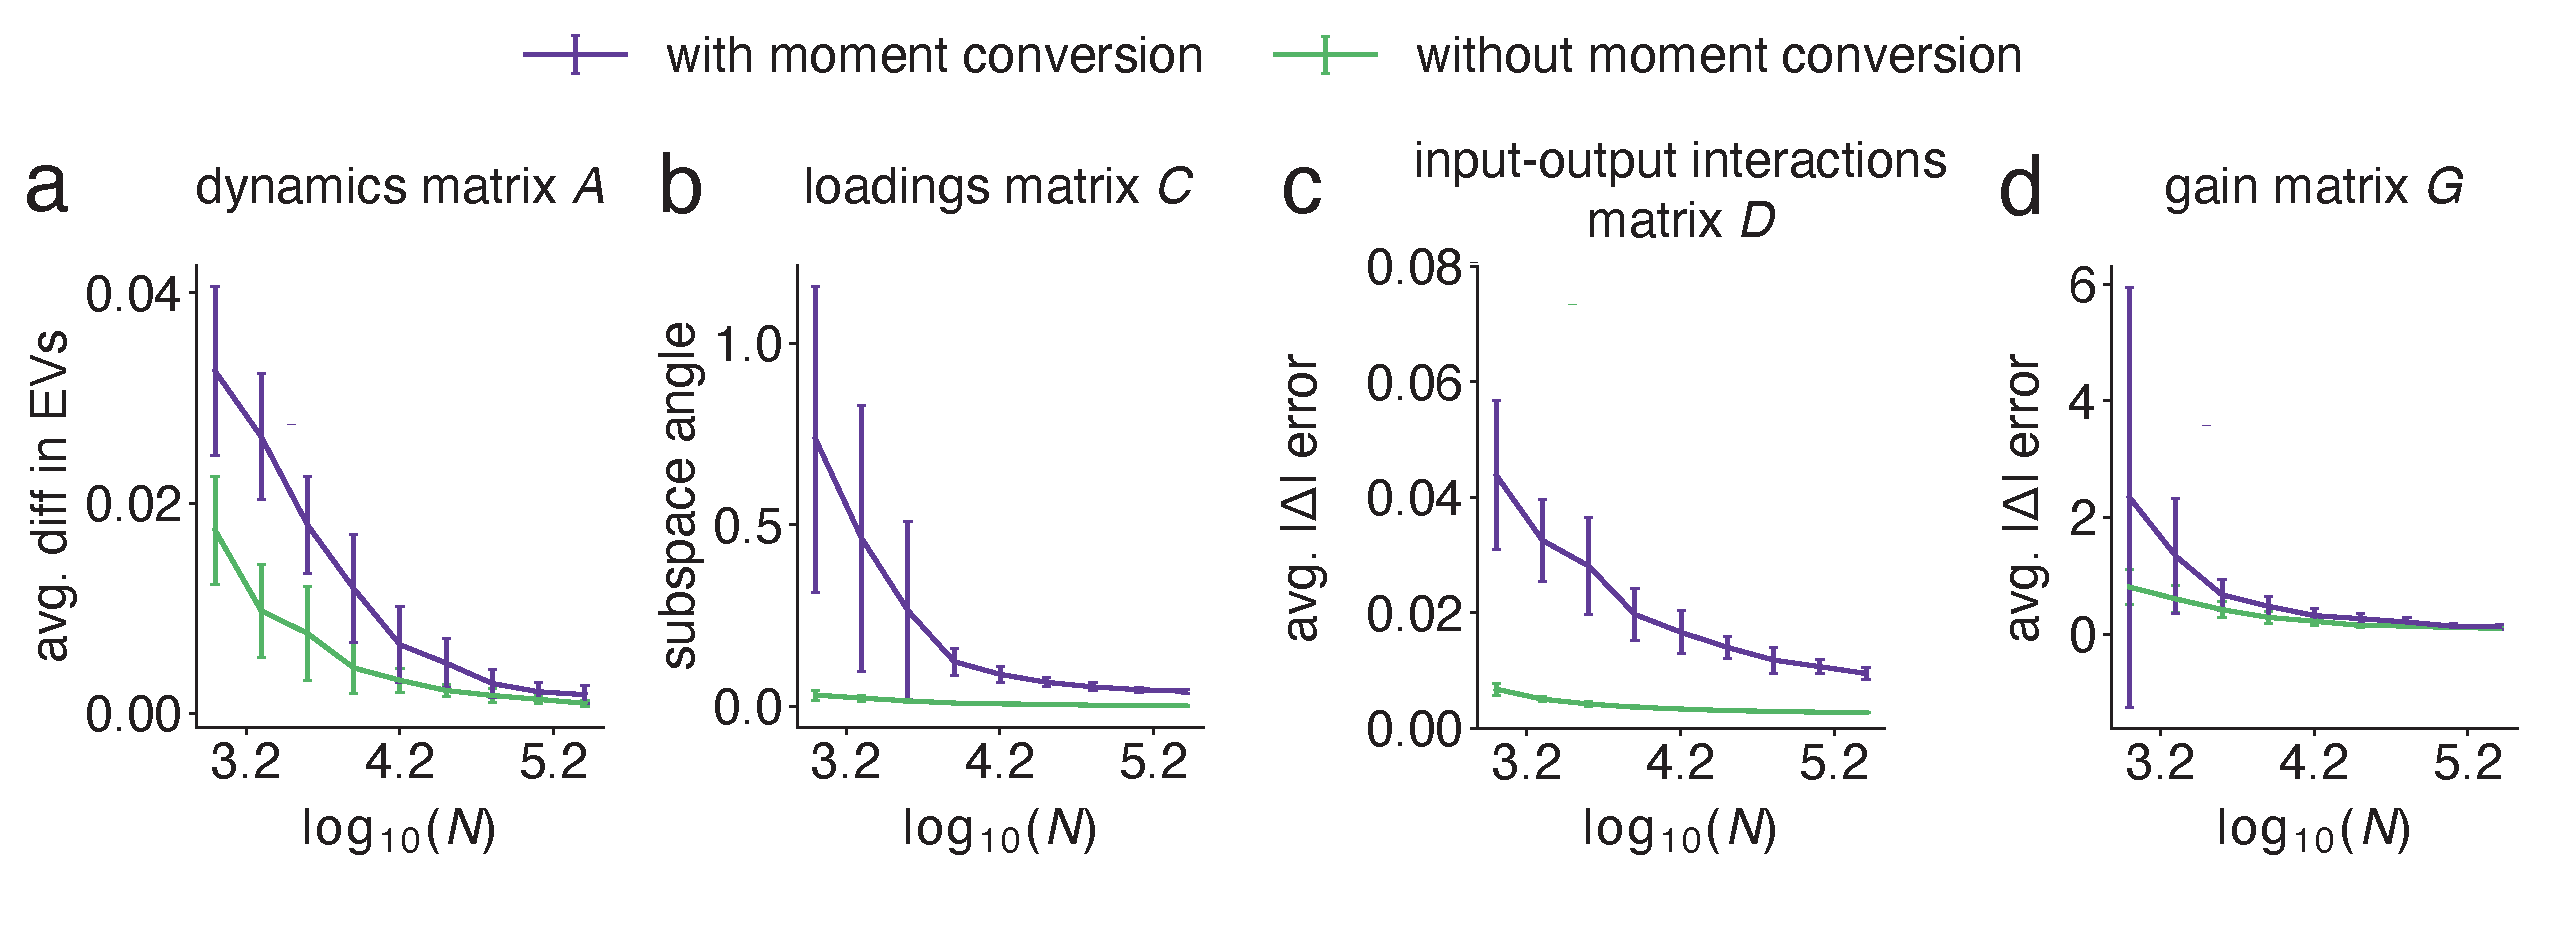
\includegraphics[width=0.90\linewidth]{ch4-bestlds/bestlds-figures/suppfig3.pdf}
\caption[bestLDS underperforms compared to a model that has direct access to $z$]{\textbf{bestLDS underperforms compared to a model that has direct access to $z$.} \textbf{(a-d)} Average recovery error for bestLDS inferred parameters (``with moment conversion'') vs. running N4SID directly on $z$ (``without moment conversion'').}
\label{fig:ap2:3}
\vspace{-0.5cm}
\end{figure*}

\begin{figure*}[ht]
\centering
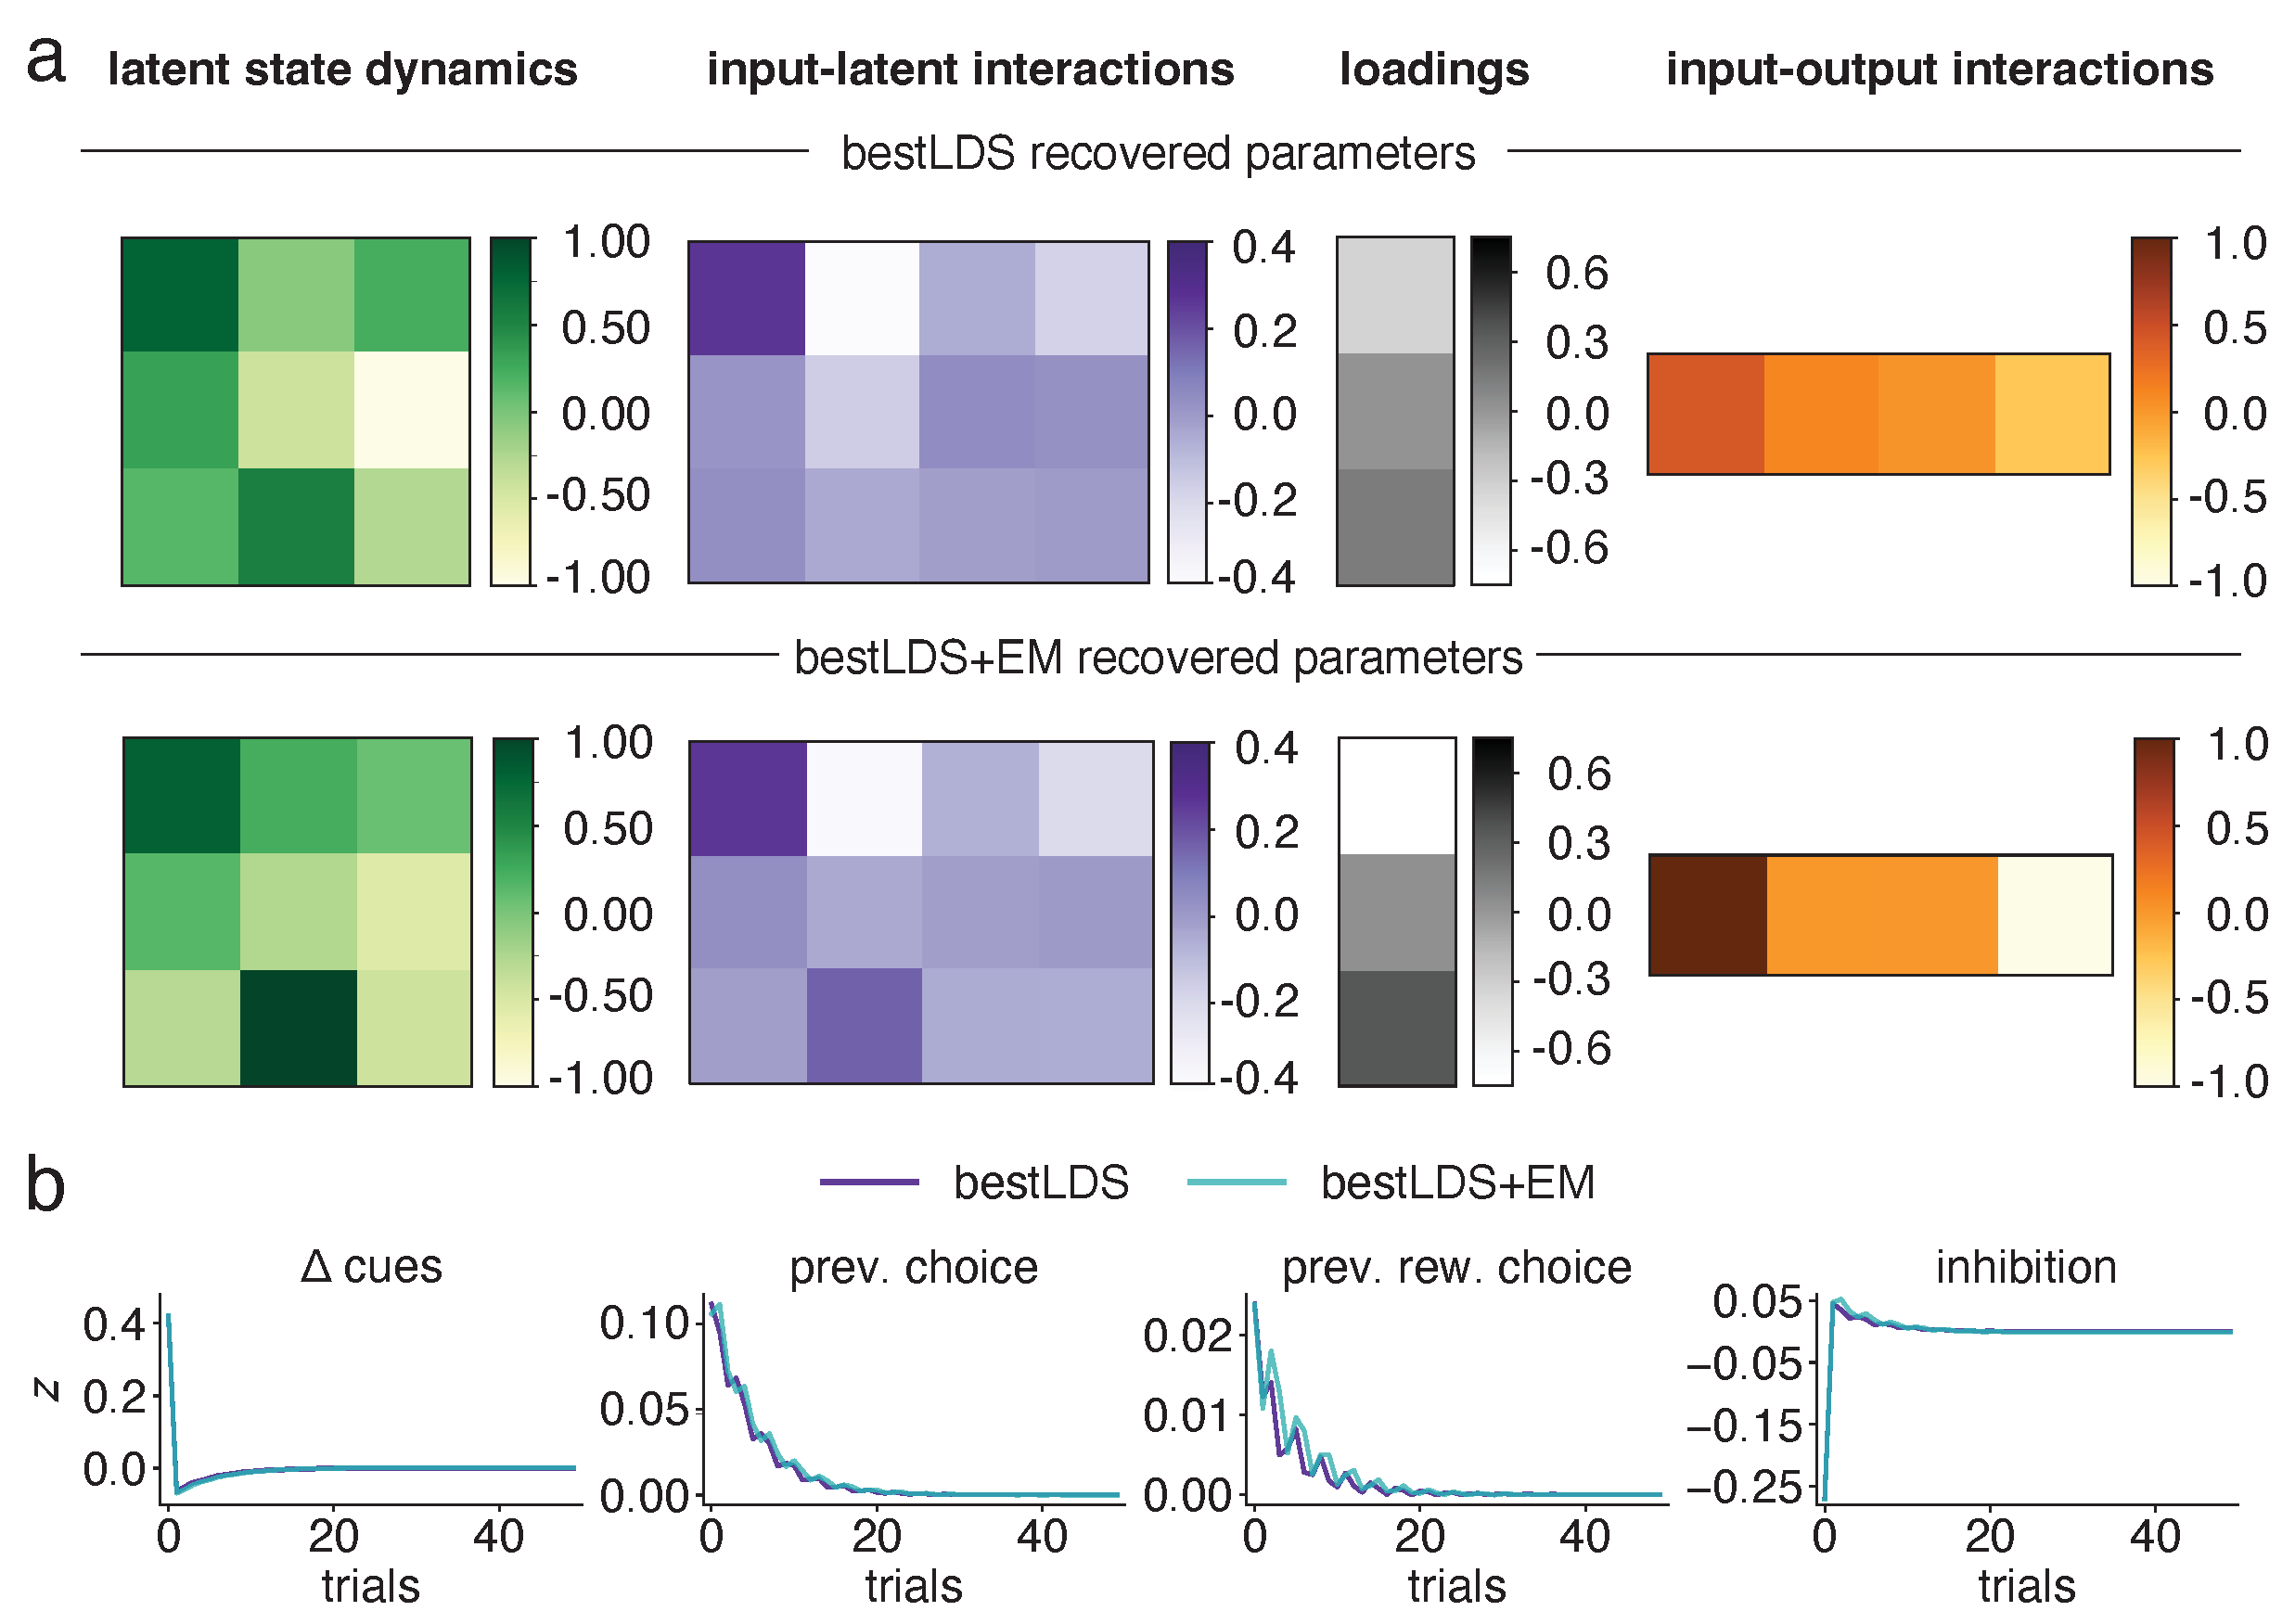
\includegraphics[width=0.95\linewidth]{ch4-bestlds/bestlds-figures/suppfig4.pdf}
\caption[bestLDS recovered parameters closely match the inferred parameters using EM with bestLDS initializations]{\textbf{bestLDS recovered parameters closely match the inferred parameters using EM with bestLDS initializations.} \textbf{(a)} The recovered parameters using bestLDS (top) and bestLDS+EM (bottom).   \textbf{(b)} Impulse responses for each of the fitted systems. In each subplot, data has been simulated noiselessly with a unit input in the indicated dimension.}
\label{fig:ap2:4}
%\vspace{-0.5cm}
\end{figure*}